\documentclass[10pt, a5paper]{article}
\usepackage{pdfpages}
\usepackage{parallel}
\usepackage[T2A]{fontenc}
\usepackage{ucs}
\usepackage[utf8x]{inputenc}
\usepackage[polish,english,russian]{babel}
\usepackage{hyperref}
\usepackage{rotating}
\usepackage[inner=2cm,top=1.8cm,outer=2cm,bottom=2.3cm,nohead]{geometry}
\usepackage{listings}
\usepackage{graphicx}
\usepackage{wrapfig}
\usepackage{longtable}
\usepackage{indentfirst}
\usepackage{array}
\newcolumntype{P}[1]{>{\raggedright\arraybackslash}p{#1}}
\frenchspacing
\usepackage{fixltx2e} %text sub- and superscripts
\usepackage{icomma} % коскі ў матэматычным рэжыме
\PreloadUnicodePage{4}

\newcommand{\longpage}{\enlargethispage{\baselineskip}}
\newcommand{\shortpage}{\enlargethispage{-\baselineskip}}

\def\switchlang#1{\expandafter\csname switchlang#1\endcsname}
\def\switchlangbe{
\let\saverefname=\refname%
\def\refname{Літаратура}%
\def\figurename{Іл.}%
}
\def\switchlangen{
\let\saverefname=\refname%
\def\refname{References}%
\def\figurename{Fig.}%
}
\def\switchlangru{
\let\saverefname=\refname%
\let\savefigurename=\figurename%
\def\refname{Литература}%
\def\figurename{Рис.}%
}

\hyphenation{admi-ni-stra-tive}
\hyphenation{ex-pe-ri-ence}
\hyphenation{fle-xi-bi-li-ty}
\hyphenation{Py-thon}
\hyphenation{ma-the-ma-ti-cal}
\hyphenation{re-ported}
\hyphenation{imp-le-menta-tions}
\hyphenation{pro-vides}
\hyphenation{en-gi-neering}
\hyphenation{com-pa-ti-bi-li-ty}
\hyphenation{im-pos-sible}
\hyphenation{desk-top}
\hyphenation{elec-tro-nic}
\hyphenation{com-pa-ny}
\hyphenation{de-ve-lop-ment}
\hyphenation{de-ve-loping}
\hyphenation{de-ve-lop}
\hyphenation{da-ta-ba-se}
\hyphenation{plat-forms}
\hyphenation{or-ga-ni-za-tion}
\hyphenation{pro-gramming}
\hyphenation{in-stru-ments}
\hyphenation{Li-nux}
\hyphenation{sour-ce}
\hyphenation{en-vi-ron-ment}
\hyphenation{Te-le-pathy}
\hyphenation{Li-nux-ov-ka}
\hyphenation{Open-BSD}
\hyphenation{Free-BSD}
\hyphenation{men-ti-on-ed}
\hyphenation{app-li-ca-tion}

\def\progref!#1!{\texttt{#1}}
\renewcommand{\arraystretch}{2} %Іначай формулы ў матрыцы зліпаюцца з лініямі
\usepackage{array}

\def\interview #1 (#2), #3, #4, #5\par{

\section[#1, #3, #4]{#1 -- #3, #4}
\def\qname{LVEE}
\def\aname{#1}
\def\q ##1\par{{\noindent \bf \qname: ##1 }\par}
\def\a{{\noindent \bf \aname: } \def\qname{L}\def\aname{#2}}
}

\def\interview* #1 (#2), #3, #4, #5\par{

\section*{#1\\{\small\rm #3, #4. #5}}

\def\qname{LVEE}
\def\aname{#1}
\def\q ##1\par{{\noindent \bf \qname: ##1 }\par}
\def\a{{\noindent \bf \aname: } \def\qname{L}\def\aname{#2}}
}


\begin{document}

\title{Использование GNU Octave для инженерных и математических расчётов}

\author{Евгений Алексеев, Оксана Чеснокова\footnote{Донецк, Украина, Донецкий национальный технический университет, \url{EAlekseev@gmail.com}}}
\maketitle

\begin{abstract}
Octave is a powerful program to solve engineering and mathe\-matical problems. Its capabilities include packages for linear algebra, analytic geometry, mathematical analysis. Octave pro\-vides rather elaborated plotting. Octave can be used to solve differential equations, optimization problems and problems of processing the experiment data, occurring frequently in engi\-neering and scientific practices.
\end{abstract}

Среди свободных математических программ наиболее известными являются Scilab и Maxima. Достойным конкурентом им может быть программа GNU Octave. Octave представляет собой  интерактивный командный интерфейс для решения математических задач. Octave "--- это мощный математический язык  интерпретирующего типа. Интерпретатор Octave входит в состав многих дистрибутивов Linux (Debian, Ubuntu, Mandriva, ALT Linux), есть версия и для ОС Windows.

Существуют и графические оболочки для работы с Octave (Qt\-Octave, Xoctave), однако главным достоинством Octave является мощный математический язык интерпретирующего типа, а также наличие постоянно пополняющегося репозитария пакетов расширений octave-forge (\url{http://octave.sourceforge.net/}).

В Octave встроен язык программирования, очень близкий к языку проприетарной программы Matlab, позволяющий  реализовать алгоритм любой сложности.

Функции Octave позволяют создавать графики и поверхности различной сложности. Для построения двумерных графиков можно использовать функции \verb!plot! и \verb!fplot!, полярные графики строятся с помощью встроенной функций \verb!polar!, функции \verb!mesh(x,y,z)!, \verb!surf(x,y,z)! позволяют строить поверхности различного вида. По умолчанию для построения графиков и поверхностей в Octave используется пакет gnuplot (\url{http://www.gnuplot.info/}), который может использоваться и как самостоятельная программа для построения графиков.

\begin{figure}[ht]
\centering{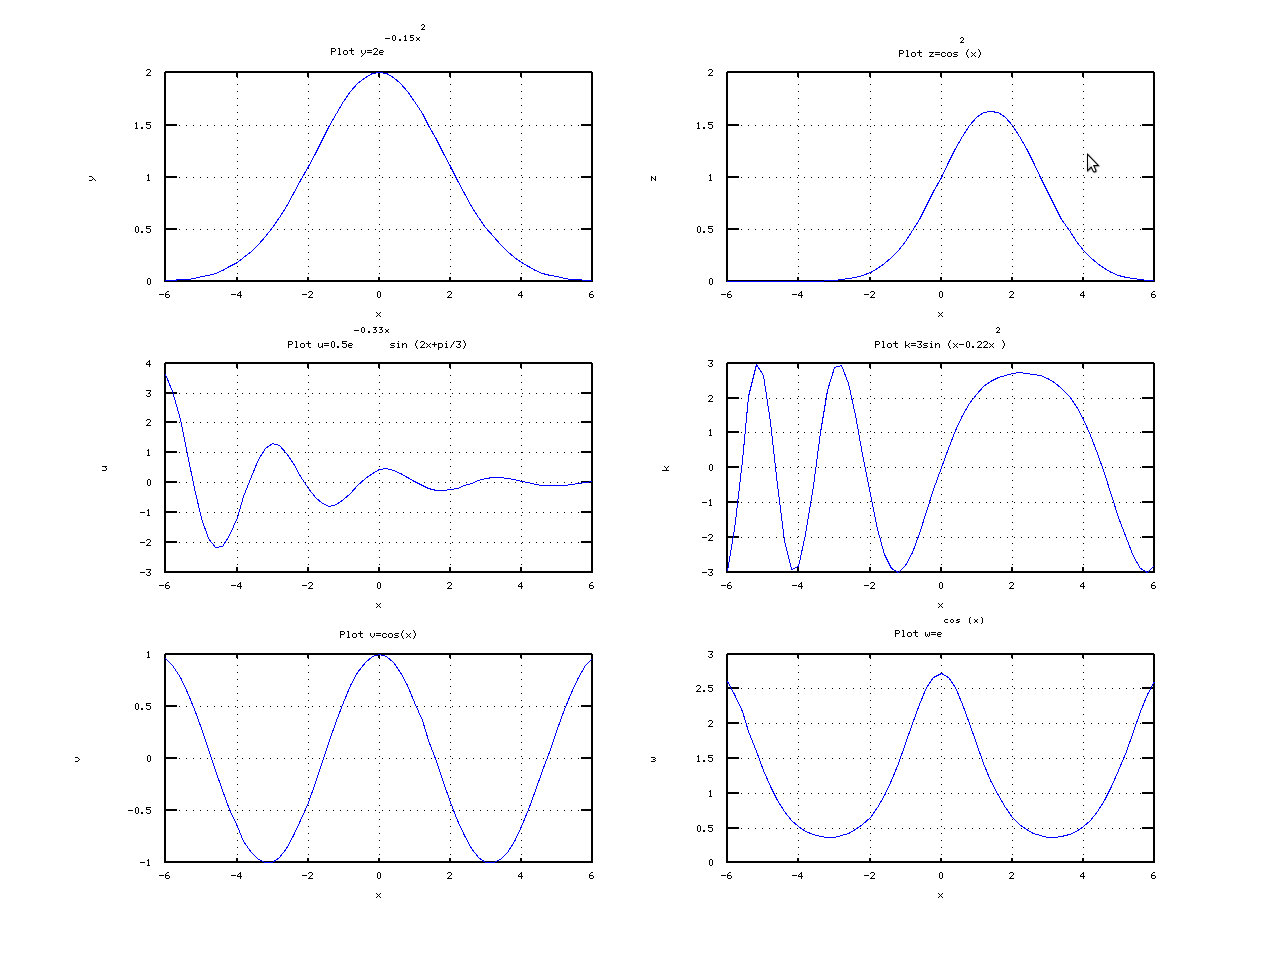
\includegraphics[width=8cm]{04_aer_octave_fig1.png}}
\caption{Графики графики нескольких функций в одном окне}
\label{pic:1}
\end{figure}

\begin{figure}[ht]
\centering{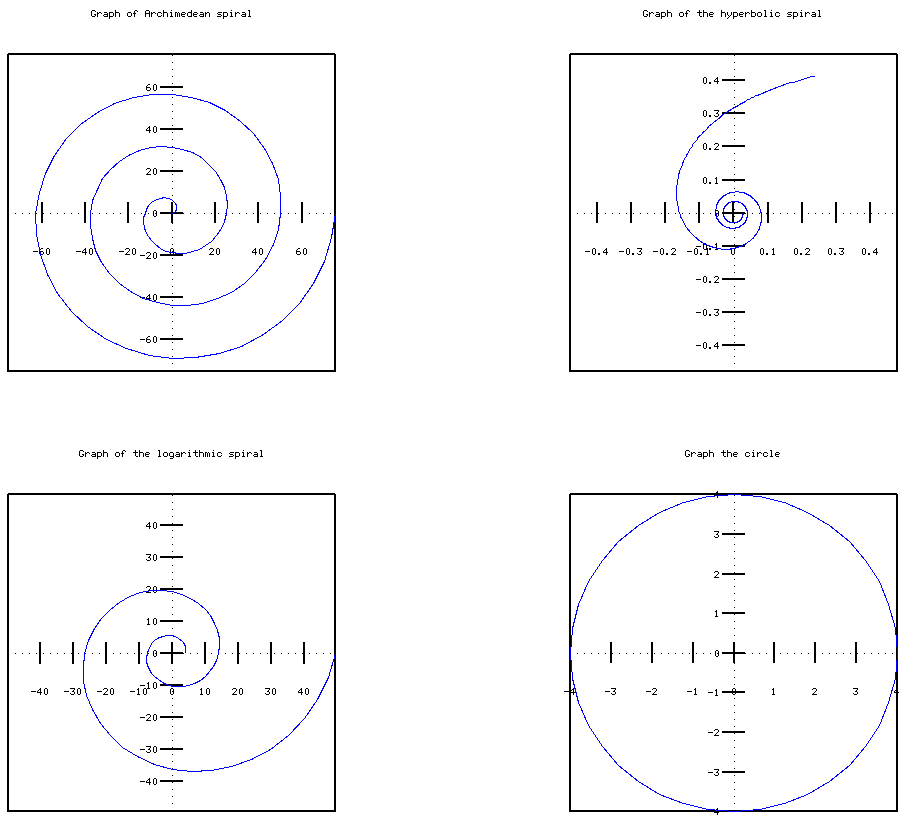
\includegraphics[width=8cm]{04_aer_octave_fig2.png}}
\caption{Графики архимедовой, гиперболической и логарифмической спирали, окружности в полярных координатах}
\label{pic:2}
\end{figure}

\begin{figure}[ht]
\centering{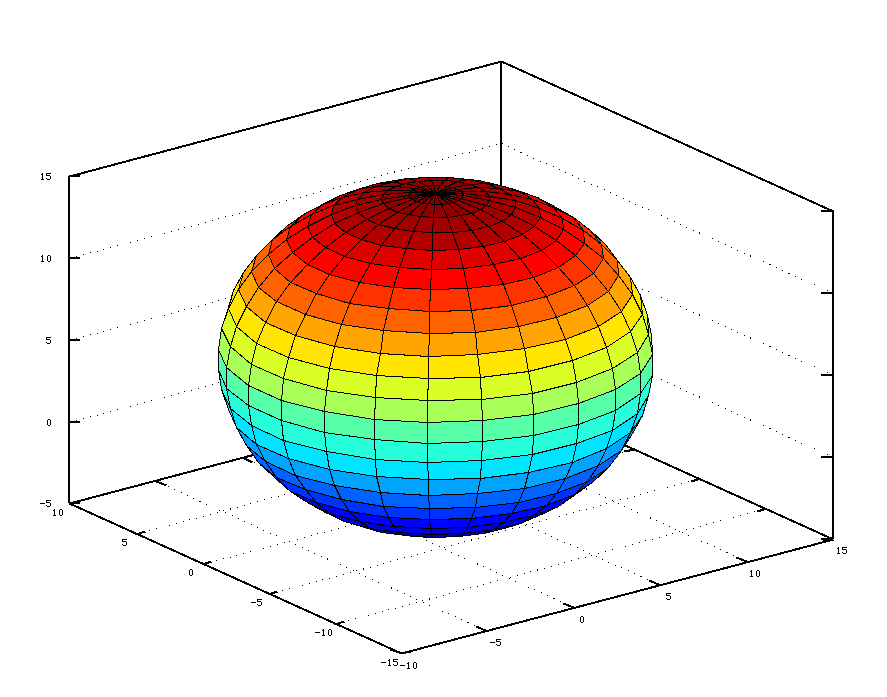
\includegraphics[width=8cm]{04_aer_octave_fig3.png}}
\caption{График сферы}
\label{pic:3}
\end{figure}

Octave содержит большое количество функций, предназначенных для решения задач линейной алгебры, наиболее используемые из них: \verb!det(M)! "--- вычисляет определитель квадратной матрицы \verb!M!, \verb!norm(M[,p])! "--- возвращает различные виды норм матрицы \verb!M! в зависимости от \verb!p!, \verb!inv(M)! "--- возвращает матрицу обратную к \verb!M!, \verb!eig(M)! "--- возвращает вектор собственных значений матрицы \verb!M!, \verb!rref(M)! "--- осуществляет приведение матрицы \verb!M! к треугольной форме, используя метод исключения Гаусса, \verb!lu(M)!, \verb!qr (M)! "--- выполняют LU и QR-разложение соответственно. 

Мощная графическая и математическая база  Octave позволяет решать задачи векторной алгебры и аналитической геометрии.

Octave содержит функции для численного и аналитического решения нелинейных уравнений и систем, а также для интегрирования и дифференцирования.

Оптимизационные задачи чаще всего решают с помощью проприетарного табличного процессора MS Excel. Однако, наиболее мощные и гибкие функции для решения подобных задач присутствуют именно в Octave. Так, для  решения линейных и нелинейных оптимизационных задач с ограничениями можно использовать функцию sqp, а для решения любых задач линейного программирования есть функция glpk. Сложные оптимизационные задачи в Octave решают с помощью пакета пакета расширений Minimization для GNU Octave (\url{http://octave.sourceforge.net/optim/overview.html}).

В инженерной практике часто приходится сталкиваться с решением обыкновенных дифференциальных уравнений и систем. В Octave существует достаточно много функций для решения обыкновенных уравнений и систем (в том числе и жёстких). Наиболее часто используемые среди них:
\begin{itemize}
\item \verb!ode23!, \verb!ode45! "--- функции решений обыкновенных нежёстких дифференциальных уравнений (или систем) методом Рунге-Кутта 2-3-го и 4-5-го порядка точности соответсвенно,
\item \verb!ode5r!, \verb!ode2r! "--- функции решений обыкновенных жёстких дифференциальных уравнений (или систем).
\end{itemize}

\begin{figure}[ht]
\centering{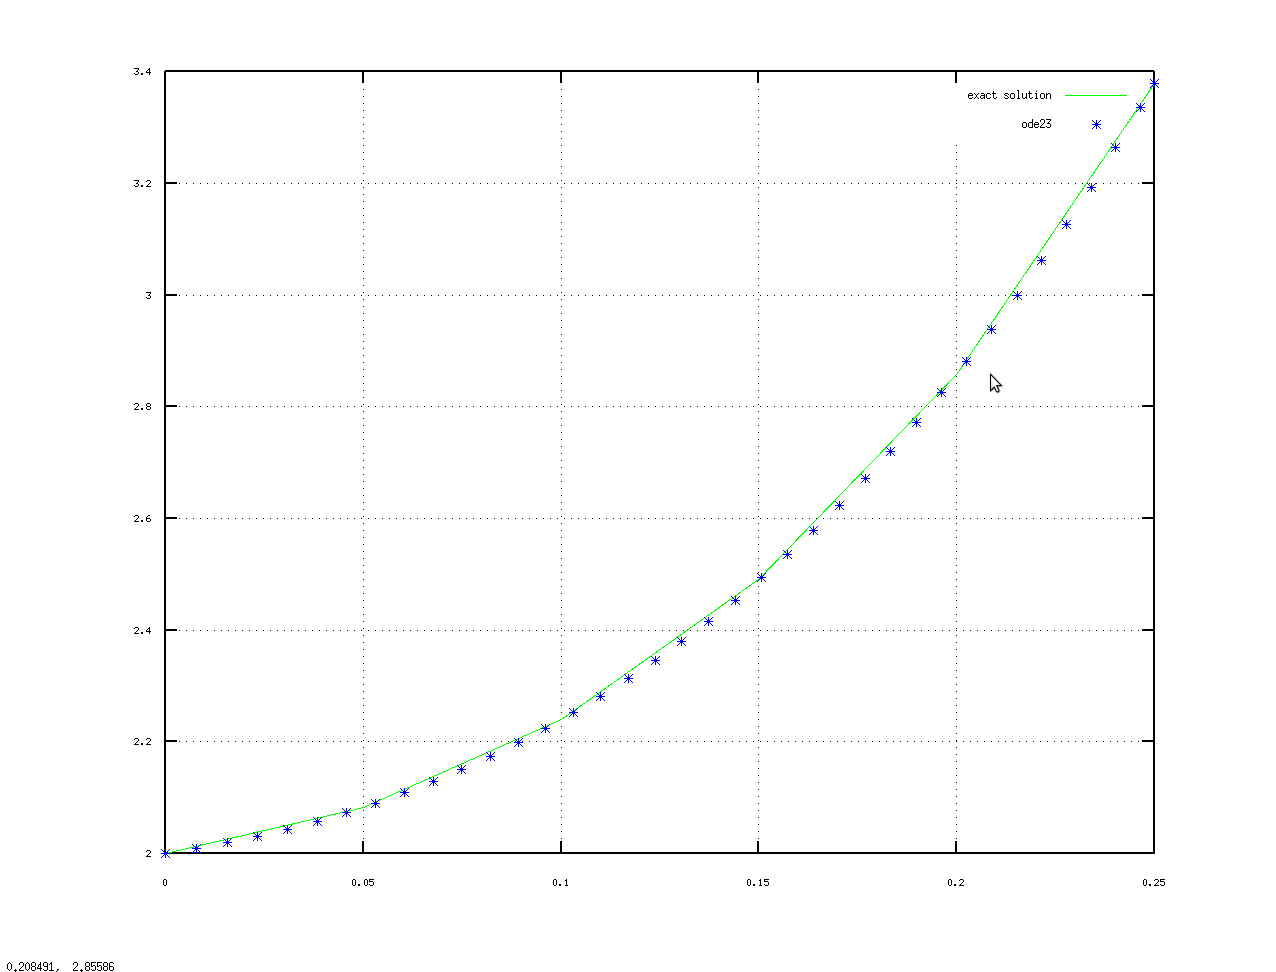
\includegraphics[width=8cm]{04_aer_octave_fig4.png}}
\caption{Графики точного решения (--) дифференциального уравнений и решения (*), найденного с помощью ode23}
\label{pic:4}
\end{figure}

Множество функций для решения дифференциальных уравнений находится в пакете расширений odepkg. Краткое описание функций этого пакета на английском языке с некоторыми примерами приведено на странице \url{http://octave.sourceforge.net/odepkg/overview.html}.

Также в Octave можно решать практически любые задачи обработки эксперимента. Для подбора параметров аналитической зависимости методом наименьших квадратов используются следующие функции: \verb!polyfit! "--- подбор коэффициентов полинома k-й степени; \verb!sqp! "--- функция поиска минимума.

Сплайн"=интерполяция в Octave реализуется с помощью функции \verb!interp1!, которая позволяет  построить кубический и линейный сплайн.

C помощью Octave можно решать и много других задач. Авторами подготовлен учебник по использованию пакете GNU Octave, который будет опубликован в ближайшее время в Москве, в серии учебников ALT Linux, а также небольшим тиражом в Донецком национальном техническом университете. Рабочие материалы книги можно увидеть на сайте \url{http://gnu-octave.narod2.ru}.

Рассмотренные возможности Octave позволяют авторам рекомендовать пакет как инструмент для решения математических задач в курсах <<Высшая математика>>, <<Математический анализ>>, <<Линейная алгебра>>, <<Аналитическая геометрия>>, а также во многих специальных курсах, в которых приходится решать задачи вычислительной математики.
\end{document}




